\chapter{Virtualización}

\section{¿Qué es la virtualización?}

La virtualización es la creación de una versión virtual (no física) de algo. Está basada en software, se puede aplicar a sistemas operativos, almacenamiento, servidores, aplicaciones, redes, etc. y es una manera de reducir gastos y aumentar eficiencia y agilidad en las empresas.

\subsection{Tipos de virtualización}

Estos son los 4 tipos de virtualización más habituales.
\subsubsection{Virtualización de servidores}

La virtualización de servidores ayuda a evitar ineficiencias ya que permite ejecutar varios sistemas operativos en una máquina física con máquinas virtuales con acceso a los recursos de todos. También permite generar un clúster de servidores en un único recurso para así mejorar mucho más la eficiencia y la reducción de costes. También permite el aumento de rendimiento de las aplicaciones y la disponibilidad al aumentar la velocidad en la carga de trabajo.

\subsubsection{Virtualización de escritorios}

La implementación de escritorios virtualizados permite ofrecer a las sucursales o empleados externos de forma rápida y sencilla un entorno de trabajo y una reducción de la inversión a la hora de gestionar cambios en éstos.

\subsubsection{Virtualización de red}

Se trata de reproducir una red física completa mediante software para poder ejecutar los mismos servicios que una red convencional y sus dispositivos. Cuentan con las mismas características y garantías que las redes físicas con las ventajas que nos ofrece la virtualización además de la liberación del hardware.

\subsubsection{Almacenamiento definido por software}

La virtualización del almacenamiento permite prescindir de los discos de los servidores. Los combina en depósitos de almacenamiento de alto rendimiento y los distribuye como software. Este nuevo modelo permite aumentar la eficiencia en el guardado de datos.
\pagebreak  

\subsection{Ventajas de la virtualización}

Como se ha podido apreciar en los tipos de virtualización presentados anteriormente, ésta conlleva una mejora considerable tanto en el rendimiento, agilidad, flexibilidad, escalabilidad, etc. como en una reducción considerable de los costes económicos y de tiempo y una simplificación en la gestión de la infraestructura.

\begin{itemize}
\item Reduce los costes de capital y los gastos operativos.
\item Minimiza o elimina los tiempos de inactividad.
\item Aumenta la productividad, la eficiencia, la agilidad y la capacidad de respuesta.
\item Implementa aplicaciones y recursos con más rapidez.
\item Garantiza la continuidad del negocio y la recuperación ante desastres.
\item Simplifica la gestión del centro de datos. 
\end{itemize}

\section{¿Qué es Docker?}

Docker es un proyecto Open Source basado en contenedores de Linux. Es básicamente un motor de contenedores que usa características del Kernel de Linux.

La idea detrás de Docker es crear contenedores ligeros y portables para las aplicaciones software que puedan ejecutarse en cualquier máquina con Docker instalado,
independientemente del sistema operativo que la máquina tenga por debajo, facilitando así también los despliegues.

De una manera más sencilla, Docker proporciona la opción de introducir
en pequeños contenedores todo aquello que nuestra aplicación necesite. Permite desplegarla en cualquier máquina que tenga Docker instalado, sin preocuparnos de nada más. 

Se podría decir que Docker son pequeñas “máquinas virtuales” pero muchos más ligeras ya que utilizan el sistema operativo de donde se ejecuta y el contenido relevante para ejecutar la aplicación está dentro de los contenedores.
\newline 

Docker es:

\begin{itemize}
\item Open-Source para la gestión de "virtualización de contenedores"
\item Aísla múltiples sistemas de archivos en el interior del mismo host
\begin{itemize}
\item Las instancias se llaman Contenedores
\item Te dan la ilusión de estar dentro de una máquina virtual
\end{itemize}
\item Piensa en entornos de ejecución o "sandboxes"
\item No hay necesidad de un hypervisor (rápido de ejecutar)
\item Requiere x64 y Linux kernel 3.8+
\end{itemize}
\pagebreak 
Docker no es:

\begin{itemize}
\item Un lenguaje de programación
\item Un sistema operativo
\item Una máquina virtual
\item Una imagen en el concepto tradicional de la máquina virtual basada en hipervisor
\end{itemize}

\section{Máquinas Virtuales vs Docker}

Las máquinas virtuales incluyen toda la aplicación, los binarios y librerías necesarias y todo un sistema operativo. Esto implica que ocupen mucho espacio, que el tiempo de ejecución sea lento y la necesidad de un Hipervisor para su utilización.

Por lo contrario, los Docker container incluyen la aplicación y todas sus dependencias pero comparten el núcleo con otros contenedores, funcionando como procesos aislados en el sistema de ficheros del sistema operativo. Los Docker container no están vinculados a ninguna infraestructura específica: se ejecutan en cualquier ordenador, en cualquier infraestructura y en cualquier cloud.

\begin{figure}[htb]
\begin{center}
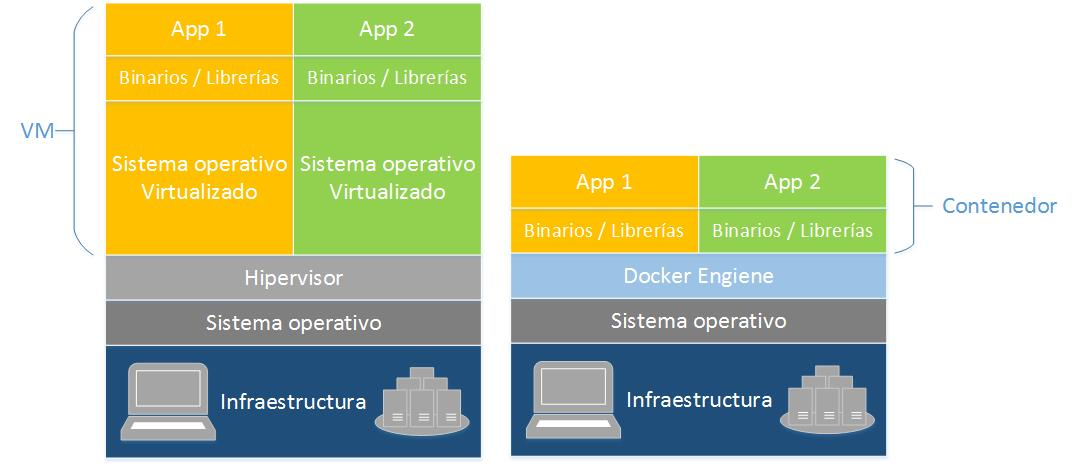
\includegraphics[width=0.8\textwidth]{./setup/VrvsDocker}
\caption{Comparativa de máquina virtual y Docker}
\label{Vs:VrvsDocker}
\end{center}
\end{figure}

En la figura \ref{Vs:VrvsDocker} se aprecian las diferencias comentadas anteriormente. La primera columna corresponde a la virtualización de 2 aplicaciones mediante la capa
intermedia del Hipervisor, el cual nos permite ejecutar los sistemas operativos virtualizados. Estos, a su vez, permiten ejecutar todos los binarios y librerías que requiere cada aplicación y, finalmente, la aplicación. La segunda columna corresponde a la contenerización de 2 aplicaciones mediante Docker Engine. Podemos observar
que no hace falta un hipervisor ya que utilizan el sistema operativo de la infraestructura
de donde son ejecutadas, pero sí son necesarios los binarios y las librerías. A simple vista se puede apreciar que, si eliminamos el sistema operativo, la infraestructura completa se hace más liviana y rápida de ejecutar.

\section{¿Por qué Docker?}\label{PqD:PQDocker}

Según lo listado en los apartados anteriores, se decidió utilizar Docker para realizar el despliegue de las aplicaciones por:

Cumplir con la condición de tecnología que pueda ser almacenada en dispositivos con una memoria reducida.

Su rapidez a la hora de levantar el servicio. En el mundo de IoT el tiempo es un bien
preciado y los sistemas se pueden apagar y encender constantemente para evitar gastos de energía innecesarios.

La facilidad para poder desplegar los servicios. Con Docker desplegar servicios es muy sencillo, solo requiere tenerlo instalado y ejecutar el contenedor para que el servicio esté activo.

La sencillez a la hora de mantener el sistema. Si hay que hacer actualizaciones o controles de una pequeña parte del servicio solo habría que cambiar o actualizar ese contenedor y no todo el sistema. Esto es un gran ahorro en recursos y tiempo. 

Por todos estos motivos se piensa que Docker puede ser una buena tecnología para desplegar sistemas de IoT. También hay que tener en cuenta que, aunque la Raspberry Pi no es un aparato con unas capacidades limitadas como podría ser un sensor utilizado normalmente, sí que cumple con todas las funciones listadas anteriormente y, por lo tanto, puede servir como preámbulo para la utilización en el resto de despliegues.  

\section{¿Cómo funciona Docker?}

En este punto se explicarán brevemente aspectos de la arquitectura, funcionamiento y
puesta en marcha de Docker.  

\subsection{Arquitectura}

Docker usa una arquitectura cliente-servidor. El cliente de Docker se comunica con el
Daemon de Docker para crear, ejecutar y distribuir los contenedores. Tanto el cliente como el Daemon pueden estar en el mismo sistema o pueden conectarse remotamente.
Como Docker usa el kernel de Linux para su ejecución, si el sistema operativo del sistema no es éste, se deberá usar una pequeña capa extra en la arquitectura de tipo VM (boot Docker) para poder correr Docker en la máquina.\newline

\subsubsection{Cliente de Docker}

Es la principal interfaz de usuario para Docker. Acepta los comandos del usuario y se
comunica con el Daemon de Docker.

\subsubsection{Imágenes de Docker (Docker Images)}

Las imágenes de Docker son plantillas de sólo lectura, que nos permitirán crear contenedores basados en su configuración.

\subsubsection{Registros de Docker (Docker Registries)}

Los registros de Docker guardan las imágenes. Éstos son repositorios públicos o privados donde se pueden subir o descargar imágenes. Sería similar a GitHub para imágenes de Docker (Docker Hub).

\subsubsection{Contenedores de Docker (Docker Containers)}

El contenedor de Docker contiene todo lo necesario para ejecutar una aplicación. Cada contenedor se crea de una imagen de Docker y es una plataforma aislada.
\newline

En la figura \ref{Inf:Infraestructura} podemos apreciar gráficamente cómo sería la arquitectura básica. El cliente podría hacer los comandos básicos de docker:

\texttt{Docker Build}: Hacer un build de un DockerFile y generar una imagen de Docker. En la figura está representado siguiendo las flechas rojas en las cuales podemos ver que el cliente se comunica con el Daemon y éste genera la imagen.

\texttt{Docker Pull}: Permite descargar una imagen de los repositorios de Docker. En la imagen se puede observar siguiendo las flechas verdes e, igual que el comando anterior, se comunica el cliente con el Daemon para que éste proceda a hacer la descarga de la imagen de mongoDB del repositorio. 

\texttt{Docker Run}: Ejecuta una imagen para generar un contendor de ésta. Siguiendo las flechas azules, veremos cómo nuevamente el cliente, al ejecutar esa comanda, se comunica con el Daemon. Este busca la imagen que se quiere ejecutar, en este caso la imagen de Ubuntu y se levanta un contenedor con la configuración de la imagen.
%\pagebreak 

\begin{figure}[htb]
\begin{center}
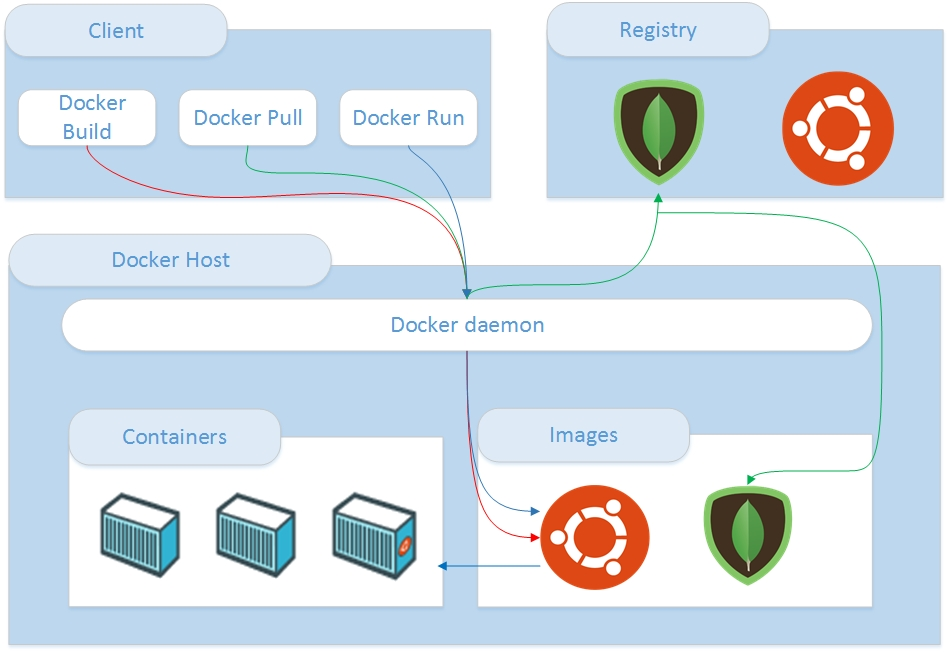
\includegraphics[width=0.69\textwidth]{./setup/Infraestructura}
\caption{Infraestructura de Docker}
\label{Inf:Infraestructura}
\end{center}
\end{figure}

\subsection{Creación de Imágenes}

Como se comenta en el punto anterior, las imágenes de Docker son las plantillas para
poder levantar los contenedores. Por eso la importancia de saber crear imágenes y personalizarlas ya que sólo permiten lectura y los cambios que hagamos en los contenedores no se verán reflejados en éstas.

La manera más sencilla de crear una imagen es descargarla del Docker Hub con el comando explicado anteriormente:

\begin{center}
\texttt{docker pull [OPTIONS] NAME[:TAG|@DIGEST]}
\end{center}

Este comando nos permite descargar una imagen en una versión concreta o tag dependiendo de nuestras necesidades. Por defecto, si no se pone nada, descargará la última. 

\begin{figure}[htb]
\begin{center}
\subfigure[Docker pull]{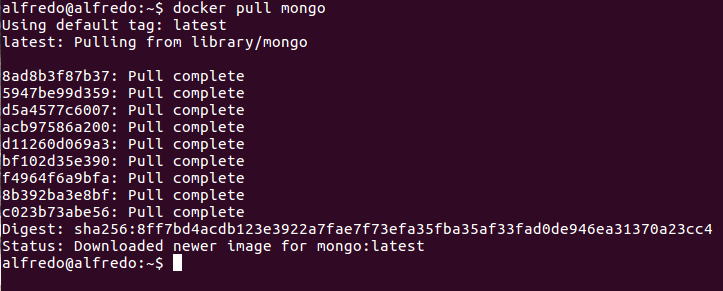
\includegraphics[width=0.90\textwidth]{./setup/DockerPull}}
\subfigure[Docker images]{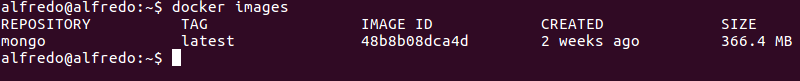
\includegraphics[width=0.90\textwidth]{./setup/DockerImages}}
\caption{Comandos de Docker (I)}
\label{Com1:ComandosDocker1}
\end{center}
\end{figure}

En la figuras \ref{Com1:ComandosDocker1} podemos apreciar como se descarga la última versión de la imagen de MongoDB y nos genera la imagen. 

Una vez obtenida la imagen se pasará a levantar el contenedor para poder ejecutar el servicio con otro de los comandos explicados. 

\begin{center}
\texttt{docker run [OPTIONS] IMAGE [COMMAND] [ARG...]}
\end{center}
\pagebreak 

\begin{figure}[htb]
\begin{center}
\subfigure[Docker ps]{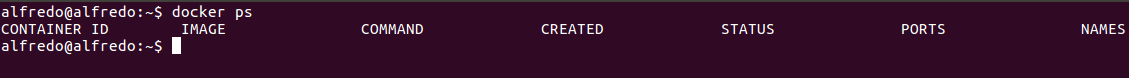
\includegraphics[width=0.90\textwidth]{./setup/DockerPs}}
\subfigure[Docker run]{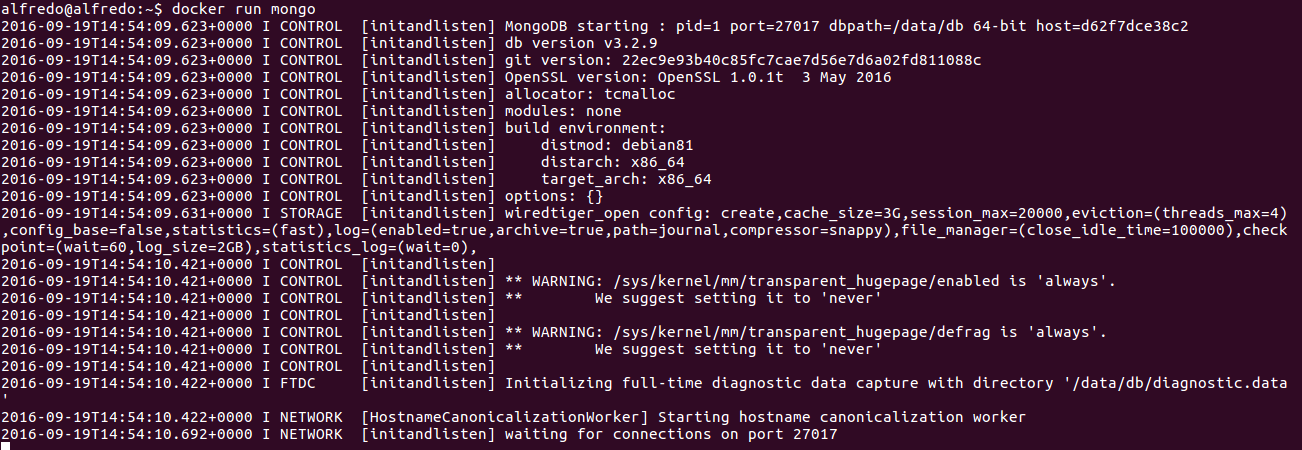
\includegraphics[width=0.90\textwidth]{./setup/DockerRun}}
\subfigure[Docker ps]{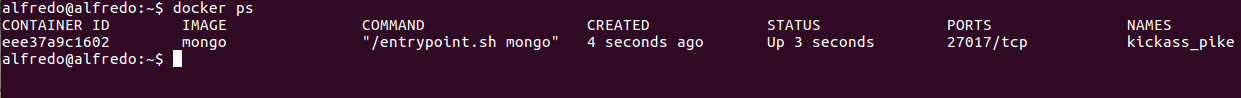
\includegraphics[width=0.90\textwidth]{./setup/DockerPsDespues}}
\caption{Comandos de Docker (II)}
\label{Com2:ComandosDocker2}
\end{center}
\end{figure}


En la figuras \ref{Com2:ComandosDocker2} se puede apreciar cómo utilizando el comando \texttt{docker ps} que
permite ver qué contenedores están levantados, no hay ninguno (a) y cómo al inicializar con el comando  \texttt{docker run mongo} levanta el servicio (b) y esta vez sí aparece el contenedor (c).

La segunda manera de crear y personalizar imágenes es mediante un \texttt{DockerFile}, que es un documento de texto donde se encuentran los comandos que se deben ejecutar para generar nuestra imagen.

El comando \texttt{docker build} comunica al Daemon de Docker que debe de leer el \texttt{DockerFile} del directorio actual y seguir las instrucciones línea por línea para la creación de nuestra imagen. Este proceso va pintando los resultados por pantalla y generando imágenes intermedias para obtener así una caché que nos permitirá en caso de errores, una vez corregido el DockerFile, continuar desde el punto conflictivo. 

\begin{verbatim}
FROM docker/whalesay:latest
CMD echo "Proyecto CoIoTe" | cowsay
\end{verbatim}

Aquí tenemos un ejemplo sencillo de DockerFile que nos servirá para explicar de una manera rápida como crearlos. 

\texttt{FROM} indica la imagen base que va a utilizar para seguir futuras instrucciones. Buscará si la imagen se encuentra localmente, en caso de que no, la descargará. En nuestro ejemplo utiliza la última versión de la imagen docker/whalesay.

La instrucción \texttt{CMD} solo puede aparecer una vez en un DockerFile, si colocamos más de uno, solo el último tendrá efecto. El objetivo de esta instrucción es proveer valores por defecto a un contenedor. Estos valores pueden incluir un ejecutable u omitir un ejecutable que en dado caso se debe especificar un punto de entrada o entrypoint en las instrucciones. En nuestro caso pintaremos un texto que se le pasara a la aplicación Cowsay.

Existen muchas más instrucciones, algunas de éstas serán explicadas más adelante cuando sea necesario su uso. 

Una vez ejecutado el comando \texttt{docker build -t docker-whale .} donde el \texttt{-t} nos permite darle nombre a la imagen y el \texttt{ .} encontrar el DockerFile para ser compilado, tal y como se ve en la Figura \ref{Build:BuildDockerFile}, descarga del repositorio la imagen ya que no la tenemos en local. Creará una imagen intermedia que nos proporciona la caché en caso de fallo, continuará con la siguiente orden creando una nueva imagen y borrando las anteriores hasta obtener la imagen definitiva. 
 
\begin{figure}[htb]
\begin{center}
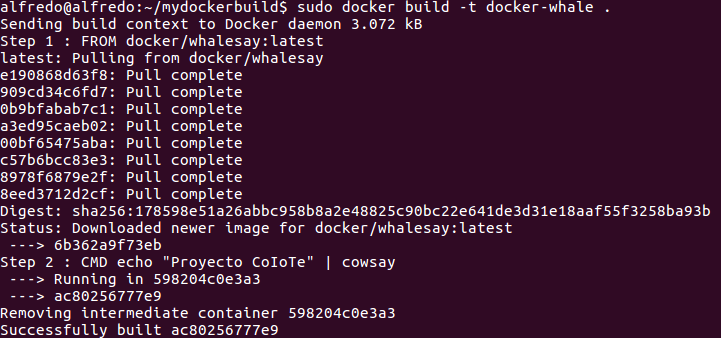
\includegraphics[width=0.90\textwidth]{./setup/DockerBuildWale}
\caption{Build del DockerFile}
\label{Build:BuildDockerFile}
\end{center}
\end{figure}
 
Una vez hecho el build del DockerFile podemos comprobar que nuestra imagen está creada correctamente (Figura \ref{Imag:ImageWhale}) y pasará a levantar el contenedor. Una vez levantado nos saldrá por pantalla el icono de Docker “diciendo” la frase que le indicamos en el fichero. (Figura \ref{Run:RunWhale}) 

\begin{figure}[htb]
\begin{center}
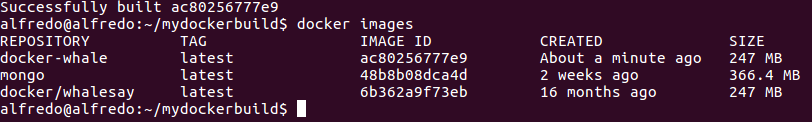
\includegraphics[width=0.90\textwidth]{./setup/DockerImagesWhale}
\caption{Docker images}
\label{Imag:ImageWhale}
\end{center}
\end{figure}
\pagebreak

\begin{figure}[htb]
\begin{center}
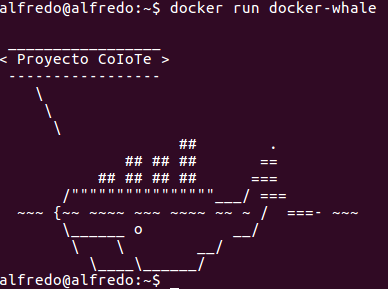
\includegraphics[width=0.50\textwidth]{./setup/DockerRunWhale}
\caption{Docker run docker-whale}
\label{Run:RunWhale}
\end{center}
\end{figure}

\subsection{Docker Compose}

Docker Compose es un orquestador que nos permite ejecutar aplicaciones que utilicen varios contenedores a la vez. Se creará un archivo docker-compose.yml donde se configurarán todos los servicios necesarios para nuestra aplicación. Una vez ejecutado este archivo nos generará todas las imágenes y con éstas los contenedores especificados a la vez que arrancará la aplicación.

Los comandos que se utilizarán serán similares a los utilizados en la creación de imágenes.

Para ejecutar el servicio y levantar todos los contenedores.

\begin{center}
\texttt{docker-compose up}
\end{center} 

Para detener el servicio y detener los contenedores.

\begin{center}
\texttt{docker-compose stop}
\end{center} 
%\pagebreak 

Docker-compose también permite ejecutar solo partes del.yml para levantar y/o detener solo algunos de los contenedores, pasándoles por parámetro el nombre del contenedor.

\begin{center}
\begin{verbatim}
version: '2'
services:
 mongo:
  container_name: mongo
  restart: always
  image: partlab/ubuntu-arm-mongodb
  volumes:
   - mongo-data:/data/db
  command: /usr/bin/mongod --smallfiles --journal
  \end{verbatim}
\pagebreak  
  \begin{verbatim}
 aaaida:
  container_name: aaaidaArm
  restart: always
  image: alteraid/aaaida-datastore-arm
  links:
   - mongo:mongo 
  environment:
   - NODE_ENV=docker
  ports:
   - "40000:40000"
volumes:\newline
 mongo-data:
   driver: local
\end{verbatim}
\end{center}

Este es un ejemplo de Docker-compose, exactamente el utilizado en el proyecto para poder levantar la infraestructura de Aaaida en la Raspberry Pi. 
La importancia en los espacios es imprescindible para que éste funcione ya que da la jerarquía adecuada para que docker-compose lo entienda.
Ahora pasaremos a explicar brevemente los argumentos que podemos encontrar en él. 
En primer lugar tenemos los servicios, en nuestro caso son 2, una base de datos MongoDB y Aaaida.

Dentro de \texttt{mongo} tendremos los siguientes: 

\texttt{container name}: Le da un nombre al contenedor para no tener que referirse a él por la id o el nombre aleatorio que proporciona Docker.

\texttt{restart}: Nos permite que en caso de fallida o reinicio del sistema este contenedor vuelva a ejecutarse.

\texttt{image}: Para poder especificar la imagen que utilizaremos para este servicio.

\texttt{volumes}: En caso de Mongo necesita un directorio donde almacenar los datos. Ésto especıfica donde se creará el volumen de datos.

\texttt{command}:  El comando que le pasamos al contenedor al momento de su ejecución. En este caso concreto es muy importante ejecutar este comando ya que activará el Journaling, que por defecto viene desactivado.

En el siguiente servicio, el de \texttt{aaaida}, a parte de disponer los mismos argumentos basicos como serian \texttt{container name}, \texttt{restart} o \texttt{image}, encontraremos alguno más como:

\texttt{links}: Define el enlace entre contenedores.

\texttt{environment}: Para poder poder pasar variables.

\texttt{ports}: Define el mapeo de puertos.

Para finalizar el archivo se encuentra los \texttt{volumes} donde se genera el volumen que hemos especificado dentro del servicio de \texttt{mongo}.  

En puntos posteriores se explicará más detenidamente el funcionamiento y la puesta en marcha del Docker Compose ya que el archivo utilizado para el ejemplo es el utilizado en la Raspberry.

\section{Conclusiones}

Como se puede observar, al virtualizar los recursos disponibles obtenemos un aumento en rendimiento y una reducción de los costes. 

Docker nos permite el despliegue de aplicaciones de una manera sencilla y en cualquier plataforma que lo soporte. 

La diferencia más significativa entre las máquinas virtuales y Docker sería el uso del Hipervisor y la necesidad de un sistema operativo para las máquinas virtuales, cosa que en Docker no es necesario. Ésto hace que las aplicaciones desplegadas de esta manera tengan una reducción en tamaño y en tiempo de ejecución.
